\documentclass[tikz,border=8pt]{standalone}
% Shared look for every TikZ diagram. Load with % Shared look for every TikZ diagram. Load with % Shared look for every TikZ diagram. Load with \input{../../tools/tikz-style.tex}
\usepackage[T1]{fontenc}
\usepackage{lmodern}
\renewcommand{\sfdefault}{lmr}  % diagrams use the same serif as the text
\usetikzlibrary{arrows.meta, positioning, shapes.geometric, calc, fit, backgrounds}
\definecolor{cblue}{HTML}{4C78A8}
\definecolor{corange}{HTML}{F58518}
\definecolor{cgreen}{HTML}{54A24B}
\definecolor{cred}{HTML}{E45756}
\definecolor{cpurple}{HTML}{B279A2}
\definecolor{cgrey}{HTML}{6B6B6B}
\tikzset{
  every picture/.style={font=\sffamily, line width=1.2pt},
  box/.style={draw=#1, fill=#1!12, rounded corners=4pt, align=center, inner sep=7pt, minimum height=1.1cm},
  box/.default=cgrey,
  arrow/.style={-{Stealth[length=3mm]}, draw=cgrey, line width=1.4pt},
  title/.style={font=\sffamily\bfseries\Large},
  note/.style={font=\sffamily\small, text=cgrey, align=center},
}
\AtBeginDocument{\hyphenpenalty=10000 \exhyphenpenalty=10000}

\usepackage[T1]{fontenc}
\usepackage{lmodern}
\renewcommand{\sfdefault}{lmr}  % diagrams use the same serif as the text
\usetikzlibrary{arrows.meta, positioning, shapes.geometric, calc, fit, backgrounds}
\definecolor{cblue}{HTML}{4C78A8}
\definecolor{corange}{HTML}{F58518}
\definecolor{cgreen}{HTML}{54A24B}
\definecolor{cred}{HTML}{E45756}
\definecolor{cpurple}{HTML}{B279A2}
\definecolor{cgrey}{HTML}{6B6B6B}
\tikzset{
  every picture/.style={font=\sffamily, line width=1.2pt},
  box/.style={draw=#1, fill=#1!12, rounded corners=4pt, align=center, inner sep=7pt, minimum height=1.1cm},
  box/.default=cgrey,
  arrow/.style={-{Stealth[length=3mm]}, draw=cgrey, line width=1.4pt},
  title/.style={font=\sffamily\bfseries\Large},
  note/.style={font=\sffamily\small, text=cgrey, align=center},
}
\AtBeginDocument{\hyphenpenalty=10000 \exhyphenpenalty=10000}

\usepackage[T1]{fontenc}
\usepackage{lmodern}
\renewcommand{\sfdefault}{lmr}  % diagrams use the same serif as the text
\usetikzlibrary{arrows.meta, positioning, shapes.geometric, calc, fit, backgrounds}
\definecolor{cblue}{HTML}{4C78A8}
\definecolor{corange}{HTML}{F58518}
\definecolor{cgreen}{HTML}{54A24B}
\definecolor{cred}{HTML}{E45756}
\definecolor{cpurple}{HTML}{B279A2}
\definecolor{cgrey}{HTML}{6B6B6B}
\tikzset{
  every picture/.style={font=\sffamily, line width=1.2pt},
  box/.style={draw=#1, fill=#1!12, rounded corners=4pt, align=center, inner sep=7pt, minimum height=1.1cm},
  box/.default=cgrey,
  arrow/.style={-{Stealth[length=3mm]}, draw=cgrey, line width=1.4pt},
  title/.style={font=\sffamily\bfseries\Large},
  note/.style={font=\sffamily\small, text=cgrey, align=center},
}
\AtBeginDocument{\hyphenpenalty=10000 \exhyphenpenalty=10000}

\begin{document}
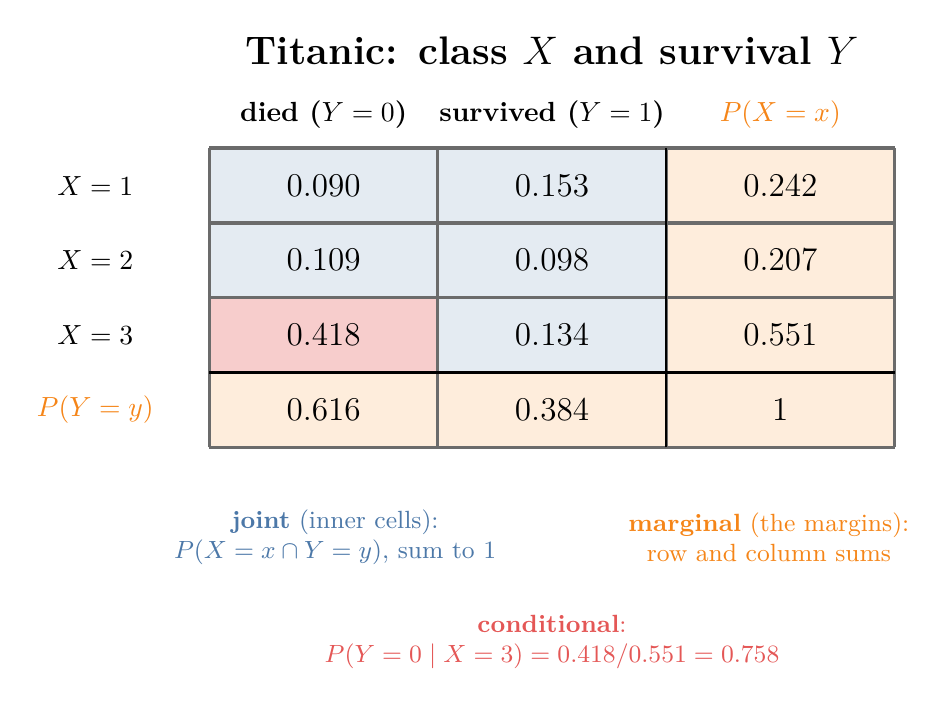
\begin{tikzpicture}[x=1cm, y=1cm]
  \def\w{2.9} \def\h{0.95}
  \node[title] at (2.5*\w,5.3*\h) {Titanic: class $X$ and survival $Y$};
  \node[font=\sffamily\bfseries] at (1.5*\w,4.45*\h) {died ($Y = 0$)};
  \node[font=\sffamily\bfseries] at (2.5*\w,4.45*\h) {survived ($Y = 1$)};
  \node[font=\sffamily\bfseries, text=corange] at (3.5*\w,4.45*\h) {$P(X = x)$};
  \foreach \c/\r in {1/3, 2/2, 3/1} \node[font=\sffamily\bfseries] at (0.5*\w,\r*\h+0.5*\h) {$X = \c$};
  \node[font=\sffamily\bfseries, text=corange] at (0.5*\w,0.5*\h) {$P(Y = y)$};
  \fill[cblue!15] (\w,\h) rectangle (3*\w,4*\h);
  \fill[corange!15] (3*\w,0) rectangle (4*\w,4*\h);
  \fill[corange!15] (\w,0) rectangle (3*\w,\h);
  \fill[cred!30] (\w,\h) rectangle (2*\w,2*\h);
  \draw[cgrey] (\w,0) grid[xstep=\w, ystep=\h] (4*\w,4*\h);
  \draw[thick] (\w,\h) -- (4*\w,\h); \draw[thick] (3*\w,0) -- (3*\w,4*\h);
  \foreach \v/\x/\y in {0.090/1/3, 0.153/2/3, 0.109/1/2, 0.098/2/2, 0.418/1/1, 0.134/2/1,
                        0.242/3/3, 0.207/3/2, 0.551/3/1, 0.616/1/0, 0.384/2/0, 1/3/0}
    \node[font=\sffamily\large] at (\x*\w+0.5*\w,\y*\h+0.5*\h) {\v};
  \node[note, text=cblue, align=center] at (1.55*\w,-1.2*\h) {\textbf{joint} (inner cells):\\ $P(X = x \cap Y = y)$, sum to 1};
  \node[note, text=corange, align=center] at (3.45*\w,-1.2*\h) {\textbf{marginal} (the margins):\\ row and column sums};
  \node[note, text=cred, align=center] at (2.5*\w,-2.6*\h) {\textbf{conditional}:\\ $P(Y = 0 \mid X = 3) = 0.418 / 0.551 = 0.758$};
\end{tikzpicture}
\end{document}
